\documentclass[letterpaper, twoside,12pt]{article}
\usepackage{amsmath}
\usepackage{amssymb}
\usepackage{graphics}
\usepackage{float}
\usepackage{tikz}
\usetikzlibrary{arrows.meta, calc, matrix, fit}
\usepackage{nicematrix}
\usepackage{colortbl}

\setlength{\parskip}{1em}

\title{Single Array Square Grid (SASQUARE)}
\date{2021-xx-xx}
\author{Kurt M. Ma. Coll}

\begin{document}
    \pagenumbering{gobble}

    \maketitle
    \newpage
    \pagenumbering{roman}

    \tableofcontents
    \newpage

    \section*{Introduction}
    In computer science, a developer uses an array to represent a series of elements of the same data type such as integers or characters. It is a data structure that holds a list of elements; each of the elements is indexed to determine its position in the list. In mathematics, the best way to represent an array is to create a row vector, a matrix with only one row. We will use a matrix because a set is unordered and does not use indices to ordinally label its elements.

    When representing an n-by-n or a square grid using arrays, a developer will intuitively use two-dimensional arrays to represent the rows and columns. In each array that represents a row, there are arrays that represent different columns. However, we can represent a square grid with only one array that can later be translated into a two-dimensional array.

    This paper aims to illustrate the conversion of a row vector with a perfect square number of elements into a perfect square matrix or vice-versa to represent a square grid.

    \newpage
    \pagenumbering{arabic}
    \section{The Square Grid} \label{1_square_grid}
    We will represent a single array with square number of indices using a row vector. The array elements shall be indexed from 1 up to the number of elements.\footnote{Programming languages, such as Python or C, often start their array indices from 0 rather than 1. Since this is a math paper, we will start with 1}
    \begin{figure}[ht]
    \centering
    \resizebox{\textwidth}{!}{%
    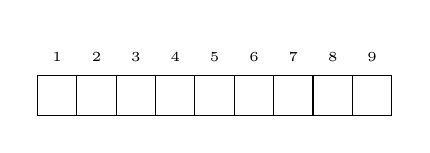
\begin{tikzpicture} [nodes in empty cells,
        nodes={minimum width=0.5cm, minimum height=0.5cm},
        row sep=-\pgflinewidth, column sep=-\pgflinewidth]
    %    border/.style={draw}
    
        \matrix(vector)[matrix of nodes, ampersand replacement=\&, % <- added ampersand replacement
        row 1/.style={nodes={draw=none, minimum width=0.3cm}},
        nodes={draw}]
        { % use \& instead of & as column separator
            \tiny{1} \& \tiny{2} \& \tiny{3} \& \tiny{4} \& \tiny{5} \& \tiny{6} \& \tiny{7} \& \tiny{8} \& \tiny{9}\\
             \& \& \& \& \& \& \& \& \\
        };
        \end{tikzpicture}%
    }
    \caption{A grid representation of a single array} \label{1f1}
    \end{figure}

    \begin{figure}[ht]
        \centering
        \resizebox{\textwidth}{!}{$
        A = 
        \begin{bmatrix}
        a_{1,1} & a_{1,2} & a_{1,3} & a_{1,4} & a_{1,5} & a_{1,6} & a_{1,7} & a_{1,8} & a_{1,9}
        \end{bmatrix}
        $}
        \caption{The array is represented as a row vector} \label{row_vector_form}
    \end{figure}

    Let $i_n$ be an array element of sequence $I$; this is the notation for an ordered list of numbers. Since the row vector has only one row, we will use this indexing notation to represent an element of the row vector. For example, we will represent the 7th element of the array as $i_7$ which is $a_{1,7}$ when indexed as an element of a row vector. The sequence form of the array in Figure \ref{row_vector_form} is:
    \begin{equation}
        A = (i_1,i_2,i_3,i_4,i_5,i_6,i_7,i_8,i_9)
    \end{equation}

    \subsection{The Base of the Square} \label{base}
    The base of a square is the root of the square. We will use it in most of the following expressions to determine particular parts of a square grid. Throughout the paper, we'll represent the base as $b$. 

    Let $b^2$ be any positive non-zero integer. The root of a perfect square can be positive or negative; for the sake of simplicity, we will use positive bases only. The number of elements in a matrix or an array is always an integer.

    \subsection{The Cells} \label{cells}
    The cells are the basic building blocks of a grid. Since a square matrix can be thought of as a grid, we will call the elements of an array or a matrix as cells. The number of cells in a square grid counts from 1 up to $b^2$ in either its row vector form or its square matrix form. We shall use integers to index each cell and call each index a cell index.

    \begin{equation}
        (i_n)^{b^2}_{n\in\mathbb{Z}^+} = (i_1, i_2, \dots ,i_{b^2})
    \end{equation}

    A square grid has rows and columns. The total number of rows in a square grid is equals to $b$ which is also equal to the total number of columns in a square grid. We will index $b$ number of rows from 1 to $b$; we will call this each index a row index. We will also do the same to the $b$ number of columns and call each index a column index. The aforementioned indices are all positive integers. Usually an array is expressed as $A_{m \times n}$ or $A_{r \times c}$. In a square matrix, $m = n$ or $r = c$. For convention, we will use $A_{r \times c}$ for expressing a square grid as a square matrix or $A_{b}$ as a row vector.

    \begin{figure}[ht]
        \centering
        \begin{minipage}{0.45\textwidth}
            \centering
            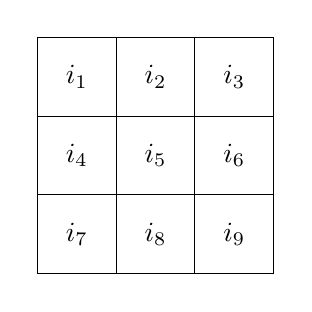
\begin{tikzpicture}
                \matrix[matrix of nodes, nodes={minimum size=1cm, draw, anchor=center}, row sep=-\pgflinewidth, column sep=-\pgflinewidth](mygrid){%
                $i_1$ & $i_2$ & $i_3$ \\
                $i_4$ & $i_5$ & $i_6$ \\
                $i_7$ & $i_8$ & $i_9$ \\
                };
            \end{tikzpicture}
        \end{minipage}
        \begin{minipage}{0.45\textwidth}
            \centering
            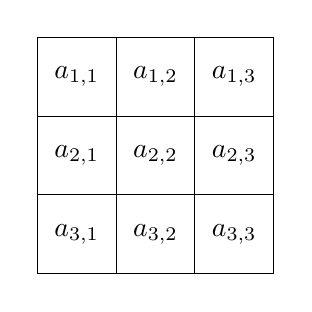
\begin{tikzpicture}
                \matrix[matrix of nodes, nodes={minimum size=1cm, draw, anchor=center}, row sep=-\pgflinewidth, column sep=-\pgflinewidth](mygrid){%
                $a_{1,1}$ & $a_{1,2}$ & $a_{1,3}$ \\
                $a_{2,1}$ & $a_{2,2}$ & $a_{2,3}$ \\
                $a_{3,1}$ & $a_{3,2}$ & $a_{3,3}$ \\
                };
            \end{tikzpicture}
        \end{minipage}

        \caption{Two square grids are labeled differently, they are indexed as elements of a sequence and a matrix respectively} \label{2forms1grid}
    \end{figure}

    In Figure \ref{2forms1grid}, the base of the square grids is 3 and the total number of cells is 9. In matrix notation, the rows and columns are indexed accordingly. We denote the elements of the right grid with $a_{r,c}$ where $r$ is the row index and $c$ is the column index. In this example, we assume that both grids represent the same array.

    \subsection{The Rows} \label{rows}
    The rows are the horizontal arrangement of elements in a matrix. In a row, there are $b$ number of cells. We shall denote a row index as $a_{r,*}$. We shall use function $r$ to determine the row of cell index $n$ in a square grid of base $b$.
    \begin{equation}
        r(b,n) = \left\lceil \frac{n}{b} \right\rceil
    \end{equation}
    We can use the function to determine which multiple of $b$ is \emph{higher} than and nearest to cell $n$ by multiplying its results to $b$. All the rightmost cells of the grid is always indexed with a number divisible by $b$. Let $a_{r,b}$ the rightmost cell index of a row.
    \begin{equation}
        a_{r,b} = b\left\lceil \frac{n}{b} \right\rceil
    \end{equation}

    \subsection{The Columns} \label{columns}
    The columns are the vertical arrangement of elements in a matrix. In a column, there are $b$ number of cells. We shall denote a column index as $a_{*,c}$. To find the column where a cell belongs, we must first identify the row where it belongs and find the rightmost cell of the row. After finding the rightmost cell of the row, we shall subtract it from the sum of the cell index $n$ and the base. We shall use function $c$.
    \begin{equation}
        c(b,n) = n + b - b\left\lceil \frac{n}{b} \right\rceil
    \end{equation}

    All the rightmost cells belong in column index $b$ which is represented as $a_{*,b}$.

    \newpage

    \subsection{Example: Row and Column of Cell 17 in 5-Square}
    \label{1_example_1}
    \begin{figure*}[ht]
        \centering
        \setcounter{MaxMatrixCols}{25}
            \tikzset{highlight/.style={
                rectangle,
                fill=gray!55,
                blend mode = multiply,
                rounded corners = 0.7 mm,
                inner sep=1pt,
                fit = #1}
            }
            \centering
            $I_5 =$
            \resizebox{\textwidth}{!}{$
            \begin{bNiceMatrix}
                i_{1} & i_{2} & i_{3} & i_{4} & i_{5} & i_{6} & i_{7} & i_{8} & i_{9} & i_{10} & i_{11} & i_{12} & i_{13} & i_{14} & i_{15} & i_{16} & i_{17} & i_{18} & i_{19} & i_{20} & i_{21} & i_{22} & i_{23} & i_{24} & i_{25}
                \CodeAfter 
                    \tikz \node [highlight=(1-17)] {};
            \end{bNiceMatrix}
            $}
    \end{figure*}

    The row vector $I$ is a square grid of base 5; to which row does cell $i_{17}$ belong to and what is the rightmost cell in that row? We shall start by using function $r$.
    \begin{equation*}
        \begin{split}
            r(b,n) &= \left\lceil \frac{n}{b} \right\rceil \\
            r(5,17) &= \left\lceil \frac{17}{5} \right\rceil \\
                &= 4
        \end{split}
    \end{equation*}

    Cell 17 belongs to row 4 . We shall substitute 4 to $r$ and 5 to $b$ in $a_{r,b}$.
    \begin{equation*}
        \begin{split}
            a_{r,b} &= b\left\lceil \frac{n}{b} \right\rceil \\
            a_{4,5} &= 5(4) \\
            a_{4,5} &= 20 \\
        \end{split}
    \end{equation*}

    The index of the rightmost cell of row 4 is 20; Cell $i_{17}$ and $i_{20}$ belong together in the same row. Next, we shall determine which column $i_{17}$ belongs to.

    \begin{equation*}
        \begin{split}
            c(b,n) &= n + b - b\left\lceil \frac{n}{b} \right\rceil \\
            c(5,17) &= 17 + 5 - 5\left\lceil \frac{17}{5} \right\rceil \\
                &= 17 + 5 - 5(4) \\
                &= 17 + 5 - 20 \\
                &= 22 - 20 \\
            c(5,17) &= 2
        \end{split}
    \end{equation*}

    \newpage

    If $i_{17}$ belongs to row $a_{4,*}$ and column $a_{*,2}$, then $i_{17} = a_{4,2}$.

    \begin{figure*}[ht]
        \centering
        \begin{minipage}{0.45\textwidth}
            \setcounter{MaxMatrixCols}{5}
                \tikzset{highlight/.style={
                    rectangle,
                    fill=gray!55,
                    blend mode = multiply,
                    rounded corners = 0.7 mm,
                    inner sep=1pt,
                    fit = #1}
                }
                \centering
                \resizebox{\textwidth}{!}{$
                I =
                \begin{bNiceMatrix}
                    i_{1} & i_{2} & i_{3} & i_{4} & i_{5} \\
                    i_{6} & i_{7} & i_{8} & i_{9} & i_{10} \\
                    i_{11} & i_{12} & i_{13} & i_{14} & i_{15} \\
                    i_{16} & i_{17} & i_{18} & i_{19} & i_{20} \\
                    i_{21} & i_{22} & i_{23} & i_{24} & i_{25}
                    \CodeAfter 
                        \tikz \node [highlight=(4-2)] {};
                \end{bNiceMatrix}
                $}
        \end{minipage}
        \hfill
        \begin{minipage}{0.45\textwidth}
            \tikzset{
                highlight/.style={
                    rectangle,
                    fill=gray!55,
                    blend mode = multiply,
                    rounded corners = 0.7 mm,
                    inner sep=1pt,
                    fit = #1
                }
            }
            \centering
            \resizebox{\textwidth}{!}{$
            =
            \begin{bNiceMatrix}
                a_{1,1} & a_{1,2} & a_{1,3} & a_{1,4} & a_{1,5} \\
                a_{2,1} & a_{2,2} & a_{2,3} & a_{2,4} & a_{2,5} \\
                a_{3,1} & a_{3,2} & a_{3,3} & a_{3,4} & a_{3,5} \\
                a_{4,1} & a_{4,2} & a_{4,3} & a_{4,4} & a_{4,5} \\
                a_{5,1} & a_{5,2} & a_{5,3} & a_{5,4} & a_{5,5}
                \CodeAfter 
                    \tikz \node [highlight=(4-2)] {};
            \end{bNiceMatrix}
            $}
        \end{minipage}
    \end{figure*}

    \newpage

    \section{The Intersection} \label{intersection}
    All cells belong to only one row and one column, hence $i_n$ can become $a_{r,c}$. An intersection is where a row and a column meet; they can only meet in one cell. The result of an intersection can be represented as either $i_n$ or $a_{r,c}$. As long as $r=c$ in matrix $A_{r \times c}$, any given pair of row and column index will always have an intersection.

    If we can determine the row and column index of a cell index with a given base, we can also determine the cell index that results of intersection a row and a column. To do so, we'll use the function $i$ which can be expressed in three ways. Let $r$ and $c$ be the row and column index respectively.
    \begin{equation}
        \begin{split}
            i(b,r,c) &= b(r-1) + c \\
                    &= br + (b - c) \\
                    &= br - b + c \\
        \end{split}
    \end{equation}
    In the first expression, the part $b(r-1)$ highlights the first $r$ rows where only $c$ number of cells are only highlighted on the last row. The second expression, highlights the $r$ number of rows then the last $(b - c)$ number of cells will be un-highlighted thereafter. The last one is the simplest form amongst the expressions.

    In the only example of Chapter \ref{1_square_grid} (Section \ref{1_example_1}), we used the functions $r$ and $c$ to determine the matrix notation for $i_{17}$ which is $a_{4,2}$. Cell index 17 belongs to row index 4 and column index 2. We shall use function $i$ to test if the intersection of $a_{4,*}$ and $a_{*,2}$ is $i_{17}$ when the $b$ is 5.
    \begin{equation*}
        \begin{split}
            i(b,r,c) &= br - b + c \\
            i(5,4,2) &= (5)(4) - (5) + (2) \\
                &= 20 - 5 + 2 \\
                &= 15 + 2 \\
            i(5,4,2) &= 17
        \end{split}
    \end{equation*}

    This function can be used to enumerate the cells in a chosen row or column.

    \newpage

    \subsection{Cells of a Row} \label{row_cells}
    To enumerate the cells of a row, we will use the Intersection function $i$. A row shall be considered a set of cell indices. Per Chapter \ref{1_square_grid}, the number of cells in a certain row is always $b$.
    \begin{equation}
        \begin{split}
            i(b,r,c) &= br - b + c \\
            a_{r,*}b &= \{ i(b,r,c) : c \in (1, \dots, b) \}
        \end{split}
    \end{equation}
    The expression $a_{r,*}b$ simply means `Row $r$ of $b$-square'. Numbers $b$ and $r$ are constants inside the set builder notation.

    \subsection{Cells of a Column} \label{column_cells}
    To enumerate the cells of a column, we will use the Intersection function $i$. Just like a row, a column is also a set of cell indices. Just like rows, a column has only $b$ number of cells.
    \begin{equation}
        \begin{split}
            i(b,r,c) &= br - b + c \\
            a_{*,c}b &= \{ i(b,r,c) : r \in (1, \dots, b) \}
        \end{split}
    \end{equation}
    The expression $a_{*,c}b$ simply means `Column $c$ of $b$-square'. Numbers $b$ and $c$ are constants inside the set builder notation.

    \subsection{Example: The Cells of Row 4 and Column 2 in 5-square} \label{2_example_1}
    To enumerate the cell indices of $a_{4,*}5$ we shall use function $i$ in a set builder notation where $r$ and $b$ is constant.
    \begin{equation*}
        \begin{split}
            i(b,r,c) &= br - b + c \\
            a_{r,*}b &= \{ i(b,r,c) : c \in (1, \dots, b) \} \\
            a_{4,*}5 &= \{ i(5,4,c) : c \in (1,2,3,4,5) \} \\
            \\
            i(5,4,1) &= (5)(4) - 5 + 1 = 16 \\
            i(5,4,2) &= (5)(4) - 5 + 2 = 17 \\
            i(5,4,3) &= (5)(4) - 5 + 3 = 18 \\
            i(5,4,4) &= (5)(4) - 5 + 4 = 19 \\
            i(5,4,5) &= (5)(4) - 5 + 5 = 20 \\
            a_{4,*}5 &= \{16, 17, 18, 19, 20 \} \\
        \end{split}
    \end{equation*}

    The set $a_{4,*}5$ has cell indices $i_{16}, i_{17}, i_{18}, i_{19}$, and $i_{20}$.

    To enumerate the cell indices of $a_{*,2}5$ we shall use function $i$ in a set builder notation where $c$ and $b$ is constant.
    \begin{equation*}
        \begin{split}
            i(b,r,c) &= br - b + c \\
            a_{r,*}b &= \{ i(b,r,c) : r \in (1, \dots, b) \} \\
            a_{4,*}5 &= \{ i(5,r,2) : r \in (1,2,3,4,5) \} \\
            \\
            i(5,1,2) &= (5)(1) - 5 + 2 = 2 \\
            i(5,2,2) &= (5)(2) - 5 + 2 = 7 \\
            i(5,3,2) &= (5)(3) - 5 + 2 = 12 \\
            i(5,4,2) &= (5)(4) - 5 + 2 = 17 \\
            i(5,5,2) &= (5)(5) - 5 + 2 = 22 \\
            a_{*,2}5 &= \{2, 7, 12, 17, 22 \} \\
        \end{split}
    \end{equation*}

    The set $a_{*,2}5$ has cell indices $i_{2}, i_{7}, i_{12}, i_{17}$, and $i_{22}$.

    Set $a_{4,*}5$ and set $a_{*,2}5$, will always meet at one cell; all pairs of $a_{r,*}b$ and $a_{*,c}b$ shall always have an intersection.

    \begin{equation*}
        \begin{split}
            a_{4,*}5 &= \{16, 17, 18, 19, 20 \} \\
            a_{*,2}5 &= \{2, 7, 12, 17, 22 \} \\
            a_{4,*}5 \cap a_{*,2}5 &= \{17\}
        \end{split}
    \end{equation*}

    The intersection of $a_{4,*}5$ and $a_{*,2}5$ is $i_{17}$ or $a_{4,2}$.

    \begin{figure*}[ht]
        \centering
        \begin{minipage}{0.45\textwidth}
            \setcounter{MaxMatrixCols}{5}
                \tikzset{row_hl/.style={
                    line width=0.8pt,
                    draw=gray!80,
                    rectangle,
                    fill=gray!55,
                    blend mode = multiply,
                    rounded corners = 0.7 mm,
                    inner sep=1pt,
                    fit = #1}
                }
                \tikzset{col_hl/.style={
                    rectangle,
                    fill=black!45,
                    blend mode = multiply,
                    rounded corners = 0.7 mm,
                    inner sep=1pt,
                    fit = #1}
                }
                \centering
                \resizebox{\textwidth}{!}{$
                I =
                \begin{bNiceMatrix}
                    i_{1} & i_{2} & i_{3} & i_{4} & i_{5} \\
                    i_{6} & i_{7} & i_{8} & i_{9} & i_{10} \\
                    i_{11} & i_{12} & i_{13} & i_{14} & i_{15} \\
                    i_{16} & i_{17} & i_{18} & i_{19} & i_{20} \\
                    i_{21} & i_{22} & i_{23} & i_{24} & i_{25}
                    \CodeAfter 
                        \tikz \node [row_hl=(4-1)(4-5)] {};
                        \tikz \node [col_hl=(1-2)(5-2)] {};
                \end{bNiceMatrix}
                $}
        \end{minipage}
        \hfill
        \begin{minipage}{0.45\textwidth}
            \tikzset{row_hl/.style={
                line width=0.8pt,
                draw=gray!80,
                rectangle,
                fill=gray!55,
                blend mode = multiply,
                rounded corners = 0.7 mm,
                inner sep=1pt,
                fit = #1}
            }
            \tikzset{col_hl/.style={
                rectangle,
                fill=black!45,
                blend mode = multiply,
                rounded corners = 0.7 mm,
                inner sep=1pt,
                fit = #1}
            }
            \centering
            \resizebox{\textwidth}{!}{$
            =
            \begin{bNiceMatrix}
                a_{1,1} & a_{1,2} & a_{1,3} & a_{1,4} & a_{1,5} \\
                a_{2,1} & a_{2,2} & a_{2,3} & a_{2,4} & a_{2,5} \\
                a_{3,1} & a_{3,2} & a_{3,3} & a_{3,4} & a_{3,5} \\
                a_{4,1} & a_{4,2} & a_{4,3} & a_{4,4} & a_{4,5} \\
                a_{5,1} & a_{5,2} & a_{5,3} & a_{5,4} & a_{5,5}
                \CodeAfter 
                \tikz \node [row_hl=(4-1)(4-5)] {};
                \tikz \node [col_hl=(1-2)(5-2)] {};
            \end{bNiceMatrix}
            $}
        \end{minipage}
    \end{figure*}

    \newpage

    \section{The Slants} \label{slants}
    A slant is a special kind of set of cells. We shall define a slant\footnote{We can also use the word `slope', but some readers may confuse it with the mathematical definition of a slope.} with these traits:
    \begin{itemize}
        \item None of the cells in the set belong in the same row
        \item None of the cells in the set belong in the same column
        \item Only one slant has $b$ number of cells; it is the longest slant
        \item Unlike rows and columns, different slants have different number of cells
        \item Two kinds of slants exist, the descending and ascending slants
    \end{itemize}

    In a square grid, there are $2b-1$ number of slants of each kind in a square grid. For example, if the square has a base of 5, there shall be 9 slants for each kind. Let $l$ be a function that takes $b$ as an argument to determine the number of slants in a square.
    \begin{equation}
        \begin{split}
            l(b) &= 2b - 1 \\
            l(5) &= 2(5) - 1 \\
            l(5) &= 9
        \end{split}
    \end{equation}

    \subsection{The Intersection Sum} \label{intersection_sum}
    There are equations that determine the slant a cell belongs to.

    By adding the row and the column index of a cell, we do an intersection sum. If two cells have the same intersection sums, they belong in the same ascending slant. Let $\sigma$ be the intersection sum function and $n$ be the cell index number.
    \begin{equation}
        \begin{split}
            \sigma(b,n) &= r(b,n) + c(b,n) \\
            r(b,n) &= \left\lceil \frac{n}{b} \right\rceil \\
            c(b,n) &= b + n - b\left\lceil \frac{n}{b} \right\rceil \\
            \sigma(b,n) &= ( \left\lceil \frac{n}{b} \right\rceil ) + (b + n - b\left\lceil \frac{n}{b} \right\rceil)\\
            \sigma(b,n) &= \left\lceil \frac{n}{b} \right\rceil + b + n - b\left\lceil \frac{n}{b} \right\rceil\\
        \end{split}
    \end{equation}

    The intersection sum is crucial to finding all the ascending slants in a square grid.
    \begin{figure}[ht]
        \centering
        {$
        \begin{bNiceMatrix}
            2 & 3 & 4 & 5 & 6 \\
            3 & 4 & 5 & 6 & 7 \\
            4 & 5 & 6 & 7 & 8 \\
            5 & 6 & 7 & 8 & 9 \\
            6 & 7 & 8 & 9 & 10
        \end{bNiceMatrix}
        $}
        \caption{This matrix has elements where $i_{n}b$ = $\sigma(b,n)$. $i_{n}b$ means cell index $n$ of $b$-square.}
    \end{figure}

    \subsection{The Intersection Difference} \label{intersection_diff}
    To do an intersection difference, we shall subtract the row index of a cell from the column index of the same cell. If two cells have the same intersection difference, they belong in the same descending slant. Let $\delta$ be the intersection difference function and $n$ be the cell index number.
    \begin{equation}
        \begin{split}
            \delta(b,n) &= c(b,n) - r(b,n)\\
            r(b,n) &= \left\lceil \frac{n}{b} \right\rceil \\
            c(b,n) &= b + n - b\left\lceil \frac{n}{b} \right\rceil \\
            \delta(b,n) &= (b + n - b\left\lceil \frac{n}{b} \right\rceil) - (\left\lceil \frac{n}{b} \right\rceil)\\
            \delta(b,n) &= b + n - b\left\lceil \frac{n}{b} \right\rceil - \left\lceil \frac{n}{b} \right\rceil\\
        \end{split}
    \end{equation}

    A reverse intersection difference occurs when we subtract the column index of a cell from the row index of the same cell. Let $\alpha$ be the reverse intersection difference.
    \begin{equation}
        \begin{split}
            \alpha(b,n) &= r(b,n) - c(b,n)\\
            r(b,n) &= \left\lceil \frac{n}{b} \right\rceil \\
            c(b,n) &= b + n - b\left\lceil \frac{n}{b} \right\rceil \\
            \alpha(b,n) &= \left\lceil \frac{n}{b} \right\rceil - (b + n - b\left\lceil \frac{n}{b} \right\rceil)\\
            \alpha(b,n) &= \left\lceil \frac{n}{b} \right\rceil - b - n + b\left\lceil \frac{n}{b} \right\rceil
        \end{split}
    \end{equation}

    A reverse intersection difference is a negated version of an intersection difference
    \begin{equation}
        \begin{split}
            \alpha(b,n) &= -(\delta(b,n))\\
            \left\lceil \frac{n}{b} \right\rceil - (b + n - b\left\lceil \frac{n}{b} \right\rceil) &= - ( b + n - b\left\lceil \frac{n}{b} \right\rceil - \left\lceil \frac{n}{b} \right\rceil)\\
            \left\lceil \frac{n}{b} \right\rceil - b - n + b\left\lceil \frac{n}{b} \right\rceil &= - b - n + b\left\lceil \frac{n}{b} \right\rceil + \left\lceil \frac{n}{b} \right\rceil\\
        \end{split}
    \end{equation}
    If we rearrange the terms of the right expression:
    \begin{equation*}
        \left\lceil \frac{n}{b} \right\rceil - b - n + b\left\lceil \frac{n}{b} \right\rceil = \left\lceil \frac{n}{b} \right\rceil - b - n + b\left\lceil \frac{n}{b} \right\rceil
    \end{equation*}

    The intersection difference is crucial to finding all the descending slants in a square grid.

    \begin{figure}[ht]
        \centering
        \begin{minipage}{0.45\textwidth}
            \centering
            {$
            A =
            \begin{bNiceMatrix}
                0 & 1 & 2 & 3 & 4 \\
                -1 & 0 & 1 & 2 & 3 \\
                -2 & -1 & 0 & 1 & 2 \\
                -3 & -2 & -1 & 0 & 1 \\
                -4 & -3 & -2 & -1 & 0
            \end{bNiceMatrix}
            $}
        \end{minipage}
        \hfill
        \begin{minipage}{0.45\textwidth}
            \centering
            {$
            B =
            \begin{bNiceMatrix}
                0 & -1 & -2 & -3 & -4 \\
                1 & 0 & -1 & -2 & -3 \\
                2 & 1 & 0 & -1 & -2 \\
                3 & 2 & 1 & 0 & -1 \\
                4 & 3 & 2 & 1 & 0
            \end{bNiceMatrix}
            $}
        \end{minipage}
        \caption{Matrix $A$ has elements where $i_{n}b = \delta(b,n)$, whilst matrix B has elements where $i_{n}b = \alpha(b,n)$.}
    \end{figure}

    \newpage

    \subsection{The Diagonals} \label{diagonals}
    A matrix has a special set of elements called a diagonal; it is also called the main diagonal. A diagonal consists of elements where $r = c$. In a square grid, a diagonal is the longest descending slant. Its two end cells are always $a_{1,1}$ and $a_{b,b}$.

    \begin{figure}[ht]
        \tikzset{highlight/.style={
            line width=0.8pt,
            draw=gray!80,
            rectangle,
            fill=gray!55,
            blend mode = multiply,
            rounded corners = 0.7 mm,
            inner sep=1pt,
            fit = #1}
        }
        \centering
        {$
        A =
        \begin{bNiceMatrix}
            a_{1,1} & a_{1,2} & a_{1,3} & a_{1,4} & a_{1,5} \\
            a_{2,1} & a_{2,2} & a_{2,3} & a_{2,4} & a_{2,5} \\
            a_{3,1} & a_{3,2} & a_{3,3} & a_{3,4} & a_{3,5} \\
            a_{4,1} & a_{4,2} & a_{4,3} & a_{4,4} & a_{4,5} \\
            a_{5,1} & a_{5,2} & a_{5,3} & a_{5,4} & a_{5,5}
            \CodeAfter 
            \tikz \node [highlight=(1-1)] {};
            \tikz \node [highlight=(2-2)] {};
            \tikz \node [highlight=(3-3)] {};
            \tikz \node [highlight=(4-4)] {};
            \tikz \node [highlight=(5-5)] {};
        \end{bNiceMatrix}
        $}
        \caption{A diagonal is highlighted in a 5-square matrix} \label{fig:diagonal}
    \end{figure}

    An anti-diagonal is the opposite of the diagonal. An anti-diagonal has cells where $r = b - c + 1$ where $b$ is the base, where $b = r + c$. The intersection sum of all its cells is always $b + 1$. It is the longest ascending slant. Its two end cells are always $a_{b,1}$ and $a_{1,b}$

    \begin{figure}[ht]
        \tikzset{highlight/.style={
            line width=0.8pt,
            draw=gray!80,
            rectangle,
            fill=gray!55,
            blend mode = multiply,
            rounded corners = 0.7 mm,
            inner sep=1pt,
            fit = #1}
        }
        \centering
        {$
        A =
        \begin{bNiceMatrix}
            a_{1,1} & a_{1,2} & a_{1,3} & a_{1,4} & a_{1,5} \\
            a_{2,1} & a_{2,2} & a_{2,3} & a_{2,4} & a_{2,5} \\
            a_{3,1} & a_{3,2} & a_{3,3} & a_{3,4} & a_{3,5} \\
            a_{4,1} & a_{4,2} & a_{4,3} & a_{4,4} & a_{4,5} \\
            a_{5,1} & a_{5,2} & a_{5,3} & a_{5,4} & a_{5,5}
            \CodeAfter 
            \tikz \node [highlight=(5-1)] {};
            \tikz \node [highlight=(4-2)] {};
            \tikz \node [highlight=(3-3)] {};
            \tikz \node [highlight=(2-4)] {};
            \tikz \node [highlight=(1-5)] {};
        \end{bNiceMatrix}
        $}
        \caption{An anti-diagonal is highlighted in a 5-square matrix} \label{fig:antidiagonal}
    \end{figure}


    \subsection{The Off-diagonal Cells} \label{offdiagonal_cells}
    The off-diagonal cells are the cells not found in the main diagonal. There are two kinds of off-diagonal cells: the superdiagonal and the subdiagonal cells. The superdiagonal cells are found above and left of the main diagonal whilst the subdiagonal cells are found below and right the main diagonal.

    Superdiagonal cells has their row index lower than their column index whilst subdiagonal cells have their row index greater than their column index. Using the intersection difference function (see section \ref{intersection_diff}), we can determine if a cell belongs to the main diagonal, is a superdiagonal cell, or is a subdiagonal cell. Given that $n$ is a cell index:
    \begin{itemize}
        \item If $\delta(b,n) < 0$, it is a subdiagonal cell.
        \item If $\delta(b,n) > 0$, it is a superdiagonal cell.
        \item If $\delta(b,n) = 0$, it belongs to the main diagonal.
    \end{itemize}

    To further illustrate the superdiagonal and subdiagonal cells, we will show two matrices where the highlighted cells together resembles two triangles.

    \begin{figure}[ht]
        \centering
        \begin{minipage}{0.45\textwidth}
            \tikzset{row_hl/.style={
            line width=0.8pt,
            draw=gray!80,
            rectangle,
            fill=gray!55,
            blend mode = multiply,
            inner sep=1pt,
            fit = #1}
            }
            \tikzset{col_hl/.style={
                rectangle,
                fill=black!45,
                blend mode = multiply,
                inner sep=1pt,
                fit = #1}
            }
            \centering
            {$
            \begin{bNiceMatrix}
                i_{1} & i_{2} & i_{3} & i_{4} & i_{5} \\
                i_{6} & i_{7} & i_{8} & i_{9} & i_{10} \\
                i_{11} & i_{12} & i_{13} & i_{14} & i_{15} \\
                i_{16} & i_{17} & i_{18} & i_{19} & i_{20} \\
                i_{21} & i_{22} & i_{23} & i_{24} & i_{25}
                \CodeAfter 
                \tikz \node [row_hl=(1-2)(1-5)] {};
                \tikz \node [row_hl=(2-3)(2-5)] {};
                \tikz \node [row_hl=(3-4)(3-5)] {};
                \tikz \node [row_hl=(4-5)] {};
                \tikz \node [col_hl=(2-1)] {};
                \tikz \node [col_hl=(3-1)(3-2)] {};
                \tikz \node [col_hl=(4-1)(4-3)] {};
                \tikz \node [col_hl=(5-1)(5-4)] {};
            \end{bNiceMatrix}
            $}
        \end{minipage}
        \hfill
        \begin{minipage}{0.45\textwidth}
            \tikzset{row_hl/.style={
            line width=0.8pt,
            draw=gray!80,
            rectangle,
            fill=gray!55,
            blend mode = multiply,
            inner sep=1pt,
            fit = #1}
            }
            \tikzset{col_hl/.style={
                rectangle,
                fill=black!45,
                blend mode = multiply,
                inner sep=1pt,
                fit = #1}
            }
            \centering
            {$
            \begin{bNiceMatrix}
                0 & 1 & 2 & 3 & 4 \\
                -1 & 0 & 1 & 2 & 3 \\
                -2 & -1 & 0 & 1 & 2 \\
                -3 & -2 & -1 & 0 & 1 \\
                -4 & -3 & -2 & -1 & 0
                \CodeAfter 
                \tikz \node [row_hl=(1-2)(1-5)] {};
                \tikz \node [row_hl=(2-3)(2-5)] {};
                \tikz \node [row_hl=(3-4)(3-5)] {};
                \tikz \node [row_hl=(4-5)] {};
                \tikz \node [col_hl=(2-1)] {};
                \tikz \node [col_hl=(3-1)(3-2)] {};
                \tikz \node [col_hl=(4-1)(4-3)] {};
                \tikz \node [col_hl=(5-1)(5-4)] {};
            \end{bNiceMatrix}
            $}
        \end{minipage}
        \caption{The cells with highlighted with a light shade of gray are the superdiagonal cells. The rest of the highlighted cells are the subdiagonal cells. The right matrix has elements where $i_{n}b = \delta(b,n)$ or $a_{r,c}b = \delta(b,n)$.} \label{fig:offdiagonal_cells}
    \end{figure}
\end{document}